\documentclass[a4paper,ukrainian,utf8,nocolumnsxix]{eskdtext}



% \newcommand{\No}{\textnumero}

\usepackage[utf8]{inputenc}
% \usepackage[english,russian,ukrainian]{babel}
\usepackage{cmap}
\usepackage[T2A]{fontenc}

\usepackage{amsmath}
\usepackage{graphicx}
\usepackage{xspace}

\usepackage{todonotes}
\usepackage{showkeys}
\usepackage[unicode]{hyperref}

\usepackage{cite}
% \usepackage{doi}


\usepackage{pdfpages}

% \usepackage{pscyr}
% \renewcommand{\rmdefault}{ftm}


\usepackage{adjustbox}




% \ESKDdepartment{Одеський національний політехнічний університет}
% \ESKDcompany{завод имени И.~А.~Лихачева}
% \ESKDclassCode{31 1398}
\ESKDtitle{Дослідження та розробка протоколів бездротових мереж на основі стандарту \iee для управління елементами індикації медіафасаду}
\ESKDdocName{}
\ESKDsignature{ІС ЗНПП 8.05010101 004 ПЗ}
\ESKDauthor{Ільїн~П.~О.}
% \ESKDtitleApprovedBy{Руководитель ОКБА}{Гусев~И.~И.}
% \ESKDtitleAgreedBy{Директор АМО ЗИЛ}{Иванов~И.~И.}
% \ESKDtitleDesignedBy{Главный инженер АМО ЗИЛ}{Петров~И.~И}
% \ESKDtitleDesignedBy{Руководитель разработки}{Лист~А.~А}

% фікси до eskd
\ESKDsectAlign{section}{Center}
\ESKDsectStyle{section}{\normalfont\MakeUppercase}
\ESKDsectStyle{subsection}{\normalfont}
\ESKDsectStyle{subsubsection}{\normalfont}

\let\stdESKDtheColumnI\ESKDtheColumnI
\renewcommand\ESKDtheColumnI{\ESKDfontIII\stdESKDtheColumnI}

\renewcommand\ESKDcolumnVIIname{Арк.}

\renewcommand\paragraph{\subsubsection}

% начать каждую секцию с новой строки
\let\stdsection\section
\renewcommand\section{\clearpage\stdsection}

% секція без номера, але в TOC
\newcommand{\sectionnonum}[1]{\section*{#1}\addcontentsline{toc}{section}{#1}}

% 
\newcommand{\figref}[1]{\figurename~\ref{#1}}

\newcommand{\iee}[0]{IEEE~802.15.4\xspace}
\newcommand{\csma}[0]{CSMA/CA\xspace}


\begin{document}
% \selectlanguage{ukrainian}


% \maketitle
\ESKDthisStyle{empty}
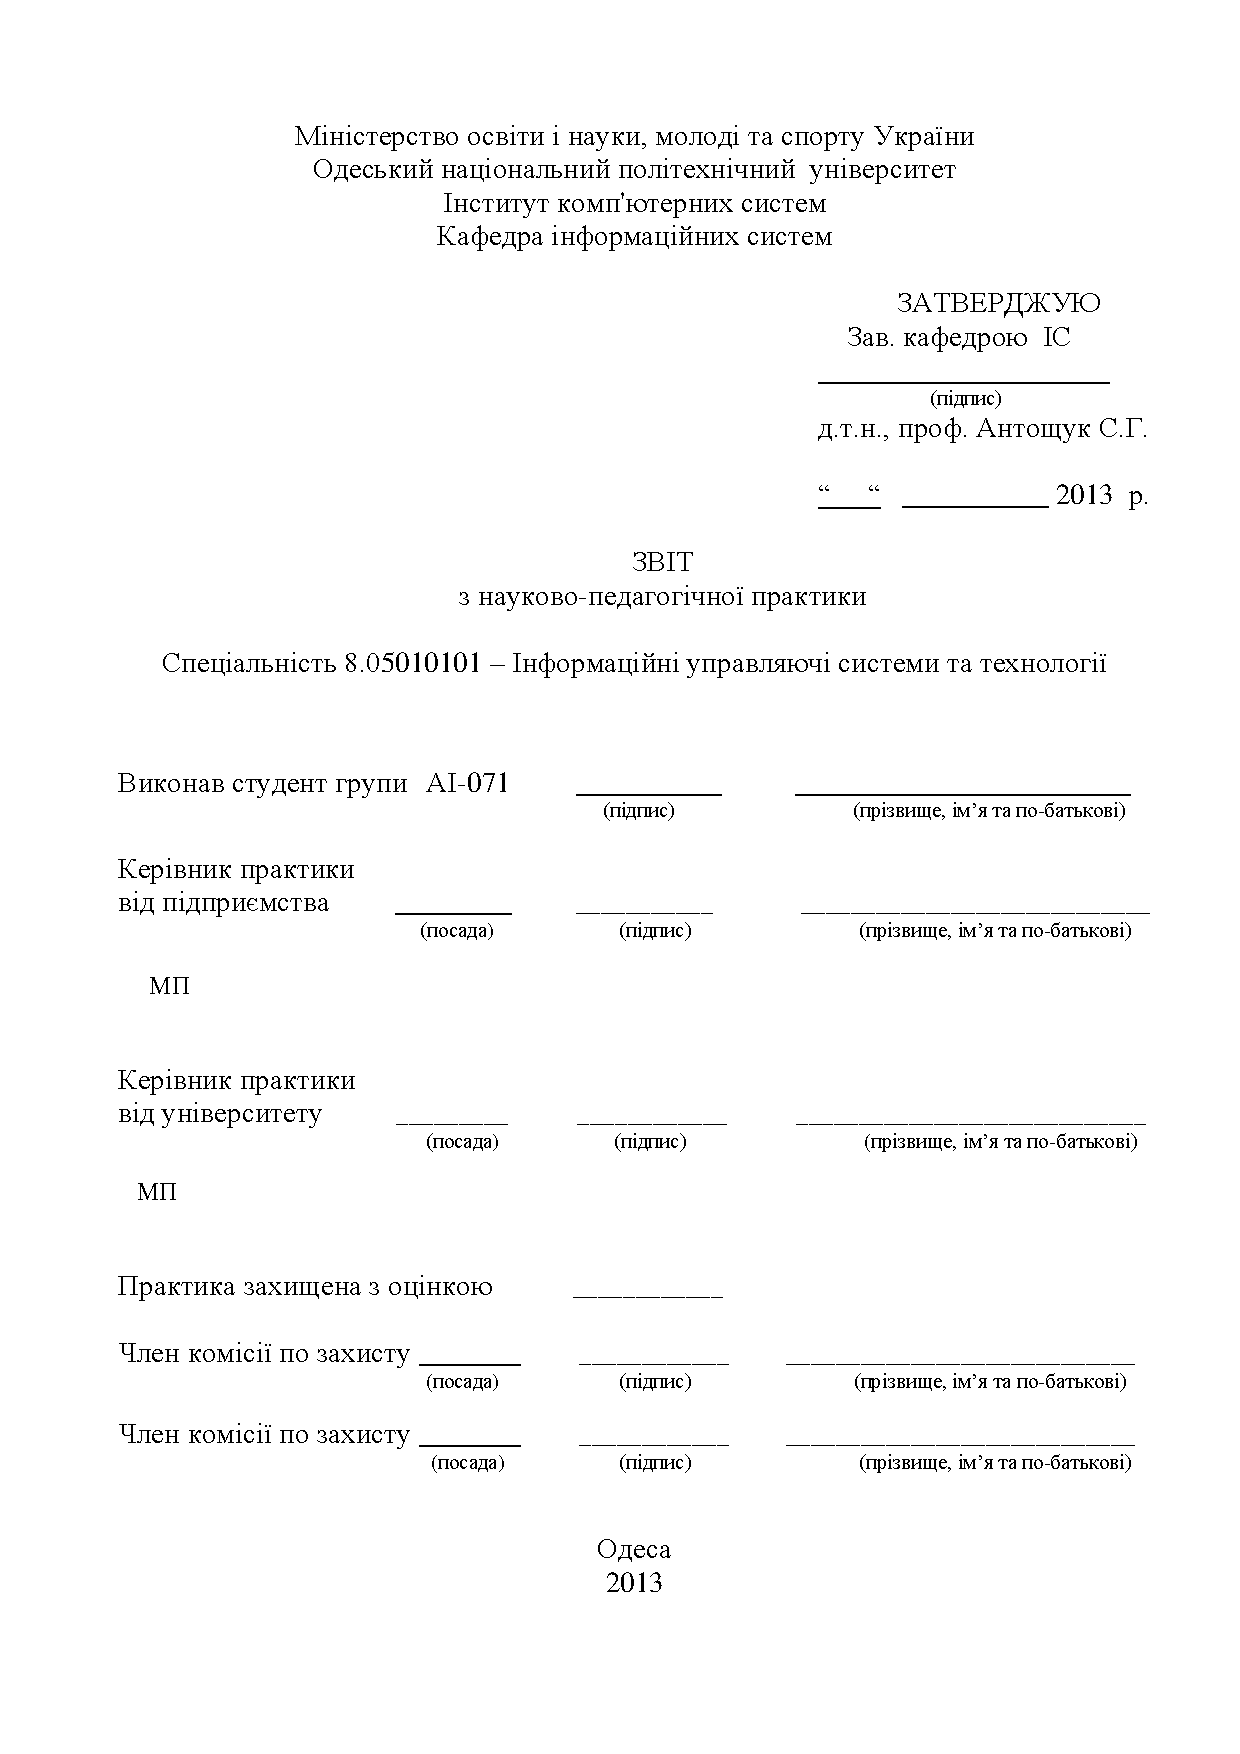
\includepdf[pages={1}]{titul/titul.pdf}

\ESKDthisStyle{formII}
\tableofcontents

% \newpage

\sectionnonum{Вступ}

Науково-педагогічна практика є заключним етапом навчання студентів у вузі і спрямована на:
\begin{itemize}
	\item розвиток навичок самостійної роботи і оволодіння методикою досліджень при розв’язанні питань, що будуть розроблятися у кваліфікаційній роботі магістрів;
	\item закріплення та розширення теоретичних і практичних знань по спеціальності, виявлення підготовленості студентів до самостійної роботи в сучасних умовах.
\end{itemize}

Метою практики є:
\begin{itemize}
	\item закріплення та розширення теоретичних і практичних знань за фахом, використання цих знань для рішення конкретних наукових, технічних, економічних та виробничих задач; 
	\item розвиток навичок самостійної практичної діяльності в умовах сучасного виробництва;
	\item придбання навиків наукової роботи;
	\item придбання навиків професійно-педагогічної діяльності;
	\item збирання та вивчення матеріалу до теми кваліфікаційної роботи магістрів.
\end{itemize}

Задачі практики:
\begin{itemize}
	\item вивчення етапів наукових досліджень та розробки засобів збору, обробки та перетворення інформації;
	\item вивчення етапів розробки та конструювання інформаційно-комп’ютерних систем;
	\item здобуття навичок розробки технічних завдань на проектування засобів вимірювання, збору, обробки та перетворення інформації, а також іншої науково-технічної документації.
	\item виконання обов’язків дублера-викладача або дублера-спеціаліста.
\end{itemize}

Я проходив переддипломну практику в якості студента-помічника в лабораторії дослідницької групи INKA при Hochschule für Technik und Wirtschaft, місто Брелін, Німеччина.

Під час проходження практики: був проведений аналіз сучасного стану підприємства, виконано індивідуальне завдання з практики, а також частково з  охорони праці. 

Індивідуальне завдання з практики відповідає темі дипломного проекту, яка  формулюється як «Дослідження та розробка протоколів бездротових мереж на основі стандарту \iee для управління елементами індикації медіафасаду». Результати можуть бути далі використані в дипломному проекті. В результаті виконання індивідуального завдання з практики був проведений огляд існуючих методів аналогів в області дослідження, запропонована методика вирішення поставленої задачі, розроблена програма на базі обраного алгоритму, проведено порівняльний аналіз та тестування системи.

\section{Індивідуальне завдання зі спеціальності}

Індивідуальне завдання з практики відповідає темі дипломного проекту, яка  формулюється як «Дослідження та розробка протоколів бездротових мереж на основі стандарту \iee для управління елементами індикації медіафасаду». Усі отримані

\subsection{Стандарт \iee}
\label{sub:ieee:standard}

Стандарт \iee було розроблено для бездротових персональних радіомереж із низькою пропускною здібністю – LR-WPAN (Low Rate Wireless Private Area Network). Перша версія стандарту була закінчена та опублікована у 2003 році. Остання ревізія стандарту була опублікована у 2011 році. 

Протягом останніх років, \iee став дуже популярним для створення WPAN і став основою для створення подальших стандартів, таких як ZigBee, 6LowPAN, WirelessHART, тощо. 

Стандарт \iee зосереджується на низько швидкісному, низько складному, енерго-ефективному бездротовому радіозв’язку серед пристроїв. Деякі з найбільш важливих особливостей стандарту є:
\begin{itemize}
	\item підтримка мережевих топологій зірка та Peer-to-Peer;
	\item використання алгоритму CSMA-CA (Carrier Sense Multiple Access with Collision Avoidance - множинний доступ з контролем несучої і униканням колізій);
	\item підтримка необов’язкового режиму доставки у реальному часі із використанням GTS (Guaranteed Time Slots – гарантованих  часових інтервалів);
	\item низькі вимоги до рівня споживання енергії;
	\item контроль споживання енергії за допомогою LQI (Link Quality Indication – показник якості зв’зку) та ED (Energy Detection – виявлення енергії).
\end{itemize}

Типово, пристрої \iee працюють в персональному просторі розміром 10 метрів чи менше. Але, робоча дальність залежить від обраного апаратного забезпечення і може досягати десятків та сотень метрів.

Бездротові канали зв’язку за стандартом \iee можуть бути встановлені на радіочастоті, що входить до діапазону ISM (Industrial, Scientifical and Medical radio bands – промислові, наукові та медичні діапазони радіочастот), який не підлягаю ліцензуванню у більшості країн. Із всіх діапазонів  ISM підтримують наступні: 2.4 ГГц, 915 МГц та 868 МГц. Підтримані діапазоні у сукупності розділені, за стандартом, на 27 каналів. 

\iee підтримує два типи пристроїв: FFD (Full-Function Device – повнофункціональний пристрій) та RFD (Reduced-Function Device – пристрій із зниженою функціональністю). RFD пристрої призначені для використання у дуже простих випадках і здібні асоціюватися лише із одним FFD. Це дозволяє втілити RFD пристрій при дуже обмеженому обсязі пам’яті, обчислювальної потужності та запасів енергії. Кожна мережа повинна містити як найменьш один FFD пристрій. 

Залежно від прикладної задачі, \iee мережа може мати топологію зірка чи  Peer-to-Peer. 

Обидва типи мереж повинні мати один спеціальний пристрій – PAN координатор. PAN координатор створює мережу, дозволяє іншим пристроям асоціювати себе із мережею та контролює доступ пристроїв до мережі у випадку використання режиму роботи із маячками (beacon-enabled mode). Тільки FFD пристрій може стати PAN координатором.

Головна різниця між мережевими топологіями полягає у напрямках комунікації, що підтримуються. Мережа-зірка підтримує комунікацію лише між PAN координатором та асоційованим пристроєм. Peer-to-Peer мережа дозволяє довільні сполучення між усіма асоційованими пристроями.

Стандарт \iee визначає два режими роботи:
\begin{itemize}
	\item режим роботи без маячків (beacon-less mode) чи безслотовий (unslotted);
	\item режим роботи із маячками (beacon-enabled mode) чи слотовий (slotted).
\end{itemize}

Розуміння цих механізмів допоможе нам розробити мережеві протоколи.


\paragraph{Режим роботи без маячків}

CSMA – це алгоритм, який використовується для контролю часу передачі в мережі, якак складається із множини пристроїв (\figref{fig:csma-ca}). Пристрої використовують контроль несучої для того, щоб визначити період часу, коли канал «вільний» і протягом котрого можливо передати інформацію. Таким чином пристрій намагається уникнути колізії. Звісно, цілком можливий випадок, коли два пристрої вирішать почати передачу  одночасно протягом одного  «вільного» періоду. Для того, щоб зменшити ймовірність цього випадку, використовується механізм випадкових періодів затримки (random back-off delay) перед початком передачі. Випадкові затримки збільшують ймовірність успішного несумісного захвату канала одним пристроєм.

\begin{figure}[bth]
	\centering
	% 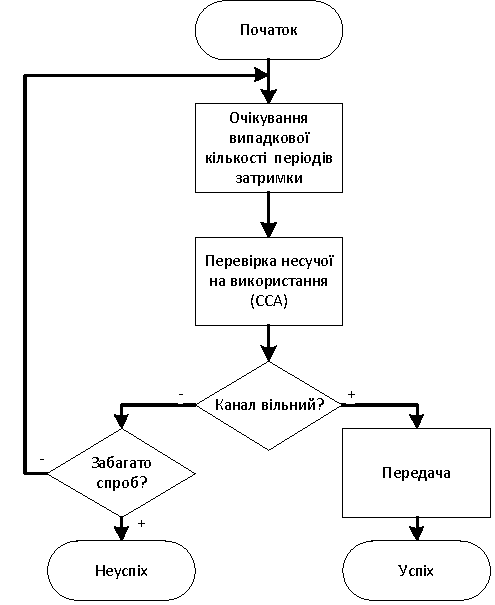
\includegraphics[width=0.7\textwidth]{img/csma-ca.pdf}
	\missingfigure{csma-ca}
	\caption{\label{fig:csma-ca}Безслотовий алгоритм \csma, спрощена версія.}
\end{figure}

У мережі, яка діє в режимі без маячків, усі пристрої використовують безслотовий алгоритм \csma. В загальному випадку, періоди затримки різних пристроїв не синхронізовані один з одним.  Кожен пристрій починає відраховувати випадковий період затримки і передачу за бажанням. Всі пристрої конкурують один з іншим за право використання каналу зв’язку. 

\paragraph{Режим роботи із маячками}
\label{par:beacon:enabled:mode}

\iee визначає додатковий, необов’язковий режим роботи із маячками. Під час цього режиму роботи, усі передачі виконуються в рамках суперкадрів (superframes). 

Кожен суперкадр складається із чотирьох частин (\figref{fig:superframe}):

\begin{itemize}
	\item маячок;
	\item CAP (Contention Access Period – період конкурентного доступу);
	\item Необов’язковий CFP (Contention Free Period – період без конкурентного доступу);
	\item Необов’язковий період неактивності.
\end{itemize}

\begin{figure}[bth]
	\centering
	% 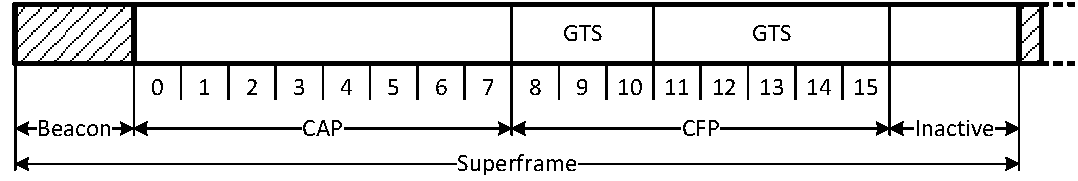
\includegraphics[width=\textwidth]{img/superframe.pdf}
	\missingfigure{}
	\caption{\label{fig:superframe}Схема суперкадру.}
\end{figure}

PAN координатор передає кадр-маячок на початку кожного суперфрейма. Інші учасники мережі використовують отриманий маячок для того, щоб синхронізуватися із координатором. Також маячок використовується для доставки опису структури поточного суперфрейму та іншої загальної інформації про мережу. 

Безпосередньо слідом за маячком починається період CAP. Протягом цього періоду усі асоційовані прилади в мережі використовують слотовий алгоритм \csma. Слотовий алгоритм \csma є модифікацією безслотового алгоритму. Пристрої так само конкурують за право передачі. Зміна полягає у наступному: якщо передача не може бути закінчена цілком до кінця періоду CAP, тоді вона взагалі не буде проведена протягом поточного періоду CAP. Замість того, вона буде відкладена до наступного. % Лише кадри підтверджень доставки та деяких інших спеціальних команд передаються без використання \csma.

Якщо PAN координатор вирішив на початку суперфрейма, що  той повинен містити необов’язковий період CFP, тоді CFP починається після закінчення періоду CAP. Координатор поділяє період CFP на гарантовані часові інтервали (GTS). Якщо пристрій бажає передати інформацію протягом періоду CFP, він повинен отримати дозвіл на це від PAN координатора за допомогою службової команди GTS Request. Дозвіл від координатора отримується протягом періоду CAP. Якщо дозвіл отримано, пристрій має виключне право на використання призначеного йому інтервалу GTS. Таким чином, протягом інтервалу GTS алгоритм \csma не використовується. Але, звісно, пристрій зобов’язаний дотримуватися границь інтервалу GTS. 

Необов’язковий період неактивності може бути назначений PAN координатором для того, щоб пристрої могли перейти до сплячого енергозберігаючого режиму. Період неактивності починається після періоду CFP (чи CAP, якщо CFP у поточному суперкадрі відсутній) і завершується із завершенням поточного суперкадру.
Негайно із завершенням поточного суперкадру починається наступний суперкадр. 

\paragraph{Оцінка пропускної здатності}
\label{par:throughput:evaluation}

Декілька досліджень було проведено для оцінки характеристик мереж на основі стандарту \iee, таких як максимальна пропускна здатність, мінімальна та максимальна затримка доставки. Дослідники використовували різноманітні підходи: теоретичні розрахунки, експерименти за допомогою симуляції математичних моделей мереж чи за допомогою справжніх мереж.

Безслотовий алгоритм \csma та режим роботи без маячків у мережах стандарту \iee був досліджений у~\cite{thoroughput:analysis:unslotted:ieee}. Цій дослід стверджує, що режим роботи без маячків має меншій рівень накладних витрат, ніж режим роботи із маячками, і тому дозволяє досягти найбільшої пропускної здатності. У досліді пропонуються аналітичні формули для оцінки значень пропускної здатності та затримки доставки. Коректність запропонованих формул була перевірена експериментально.

Дослід~\cite{thoroughput:analysis:unslotted:ieee} пропонує оцінювати корисну пропускну здібність як функцію від розміру корисного навантаження кадру (\figref{fig:throughput_graph}). За допомогою розрахунків встановлено, що верхня межа корисної пропускної здібності в мережі, яка використовує 16 біт для адресування, сягає рівню 151 кбіт/с із відключеним механізмом підтверджень чи рівню 139 кбіт/с – із включеним. Із зменшенням розміру корисного навантаження кадру, корисна пропускна здібність також зменшується. Розмір заголовку кадру (і, відповідно, можливий розмір корисного навантаження) змінюється відповідно до обраного режиму адресування та параметрів безпеки. Тобто, максимальна корисна пропускна здібність залежить від обраних параметрів мережі.

\begin{figure}[bth]
	\centering
	% 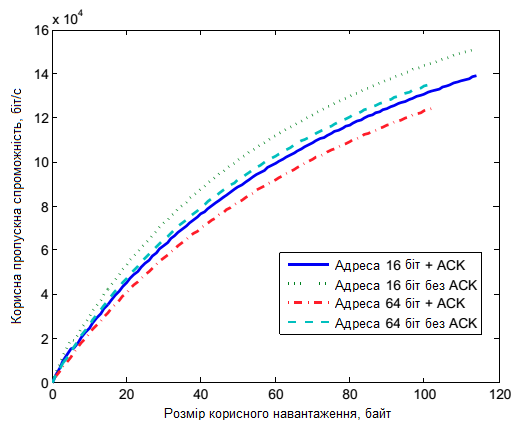
\includegraphics[width=0.7\textwidth]{img/throughput_graph.png}
	\missingfigure{}
	\caption{\label{fig:throughput_graph}Корисна пропускна здібність як функція корисного навантаження, режиму адресування та найстройок підтвердження доставки (ACK).}
\end{figure}

Експерименти, що були проведені у досліді~\cite{thoroughput:analysis:unslotted:ieee}, показують стабільну різницю між оціненою та експериментально виміряною корисною пропускною здібністю. Виміряна корисна пропускна здібність була десть на 11\% нижче за очиковану, тобто максимально досягнута пропускна здібність становила біля 123 кбіт/с.

The prototype of the system, which was built during Forschungsproject 1, was also used to measure a useful bitrate. The prototype have used the MRF24J40MA transceivers, installed on Arduino Leonardo boards. During the experiment, the usefull bitrate level have reached 110~kbit/s. This result corresponds to the results, obtained in the~\cite{thoroughput:analysis:unslotted:ieee}.%\todo{link to the test source}

Слотовий алгоритм \csma та режим роботи із маячками у мережах стандарту \iee був досліджений в ~\cite{simulation:study:slotted:ieee} та в ~\cite{gts:allocation:analysis}. Серед іншого, ці досліди встановлюють взаємозв'язок між порядком суперкадра (superframe order, розмір суперкадра) та максимальною пропускною здібністю. Досліди стверджують, що пропускна здібніть сягає свого здійснимого максимуму, якщо порядок суперкадру дорівнює 3 або 4. При більших порядках, пропускна здібність зменшується.

Аналіз та порівняння слотового та безслотового алгоритмів \csma в стандарті \iee було проведено в ~\cite{analysis:slotted:unslotted}. У висновках досліду зазначається, що безслотовий алгоритм \csma  показує більшу максимальну пропускну здібність у порівнянні із слотовим алгоритмом \csma.

Але, цей висновок не є підставою для того, щоб вважати режим роботи із маячками, який використовує слотовий алгоритм \csma, повністю непотрібним. Цей режим пропонує дуже важливі особливості, які можуть бути використані для розробки мережевіх протоколів специфічних для прикладної програми.

\subsection{Мережевий протокол для системи медіа фасаду}
\label{sub:network:protocol:amf}


Ця глава присвячена розробці мережевого протоколу для системи медіа фасаду.

\paragraph{Архітектура системи}
\label{par:system:arch}

Перед усім, розглянемо архітектуру системи ад-хок медіа фасаду (\figref{fig:sys_arch}). 

\begin{figure}[bth]
\centering
\adjustbox{max width=\textwidth}{
	% %!TEX root = ../praktika.tex


\begin{tikzpicture}[auto, node distance=6em,]

	\tikzstyle{block}=[draw, text width=5.7em, text centered, minimum height=3em, fill=white]

	\begin{pgfonlayer}{foreground}
		\node[block] (hc) {Хост-контролер};
		\node[block, below of=hc] (ha) {Хост-додаток};
		\node[block, right of=ha, node distance=10em] (ra) {Вiддалений додаток};
		\node[block, right of=hc, node distance=10em] (ln) {Вузел};

		\draw[thick,<->] (hc.south) -- (ha.north);
		\draw[thick,<->] (ha.east) -- (ra.west);
		\draw[thick,<->] (hc) -- (ln);

		\path (hc.west) -- (ln.east)
			 node[pos=0.5](betw-hc-ln) {} ;

		\node[block, above of=betw-hc-ln, text width=10em, node distance=4em] (sen) {Сенсори};

		\draw[thick,->] (sen) -- (hc);
		\draw[thick,->] (ln) -- (sen);
	\end{pgfonlayer}

	\begin{pgfonlayer}{background}
		\path (hc.west |- sen.north)+(-0.5,0.8) node (a) {};
		\path (ha.east |- ha.south)+(0.5,-0.3) node (b) {};
		\path[draw] (a) rectangle (b);
	
		\path (ln.west |- sen.north)+(-0.5,0.8) node (c) {};
		\path (ln.east |- ln.south)+(0.5,-0.3) node (d) {};
		\path[draw] (c) rectangle (d);
	\end{pgfonlayer}

	\begin{pgfonlayer}{foreground}
		\draw[] (a) node[anchor=north west] (host-label) {Хост};
		\path[draw] (host-label.south west) -- (host-label.south east) -- (host-label.north east);
		
		\draw[] (c) node[anchor=north west] (node-label) {Вузел};
		\path[draw] (node-label.south west) -- (node-label.south east) -- (node-label.north east);
	\end{pgfonlayer}

\end{tikzpicture}

	\missingfigure{}
}
\caption{\label{fig:sys_arch}Загальна архитектура системи}
\end{figure}

Система поділяється на дві основні частини: Хост та Вузли візуалізації.

Вузли візуалізації виконують, перед усім, фактичну роботу по візуалізації, а також дозволяють користувачам системи взаємодіяти із системою. Вузли можуть мати необов’язкові сенсори, які можуть використовуватися системою для визначення положення Вузлів та інших видів взаємодії із користувачами.

До складу Хоста входять Хост-контролер, Хост-додаток та сенсори. Сенсори на стороні Хоста використовуються для визначення положення Вузлів. Хост-додаток проводить загальне керування візуалізацією, системою. Хост-контролер використовує інформацію від сенсорів для того, щоб розподілити керівні команди від Хост-додатка на окремі завдання для Вузлів. Хост-контролер проводить оновлення візуалізації, посилаючи необхідні команди Вузлам через канал зв’язку.

Блок Віддалений додаток представляє на схемі будь яку іншу систему, яка під’єднана до системи медіа-фасаду, але не приймає активної участі в процесі візуалізації. Це може, наприклад, бути деякий інтерфейс користувача для адміністрування системи, Web-додаток, сусідня система візуалізації, тощо.

Згідно з запропонованою архітектурою системи, Вузли візуалізації не підтримують зв’язок один з одним заради цілей прикладної системи, візуалізації. Вузли спілкуються лише із Хост-контролером, щоб отримати оновлення візуалізації, повідомити інформацію з сенсорів. Однак, спілкування між Вузлами заради цілей управління мережею знаходиться поза рамками запропонованої архітектури і не забороняється.

\paragraph{Випадки трафіку}
\label{par:traffic:cases}

Виходячи із наведеної в пункті~\ref{par:system:arch} архітектури системи, можна виділити два види мережевого трафіку в системі:
\begin{itemize}
	\item Трафік від Хоста к Вузлам;
	\item Трафік від Вузлів к Хосту.
\end{itemize}

Обидва види не однорідні і складаються с команд та даних різного роду, розміру та вимог до QoS (Quality of Service – якість обслуговування). QoS – це гарантії від мережі до прикладної програми щодо якості характеристик каналу зв’язку: пропускна здібність, час доставки.

Трафік від Хоста к Вузлам складається, перед усім, з команд оновлення візуалізації. Ці команди змінюють візуальний стан Вузлів. Залежно від типу, природи візуалізації, до цього виду трафіка можуть пред’являтися різні вимоги щодо часу і гарантій доставки. Але, можна очікувати, що команди візуалізації будуть складати основну частину всього мережевого трафіку.

Одним з найпростіших для виконання механізмів оновлення візуалізаціє є наступний: усі Вузли оновлюються часто і одночасно, так само, як окремі пікселі на моніторі оновлюються одночасно при зміні кадру. При цьому механізмі, команди на оновлення відсилаються часто. В такому випадку, витрата однієї команди на оновлення буде менш помітна і менш впливова на загальний опит користувача. Більш важливою є доставка  команд оновлення у встановлені рамки ніж надійна доставка. Якщо команда запізнюється із доставкою – її все одно можна відкидати, бо вона застаріла і скоро прийде наступна. Цей підхід використовується в існуючих протоколах потокової передачі медіа-контенту. Звісно, якщо кількість відкинутих чи втрачених пакетів завелика, тоді якість сигналу падає аж до рівню повної непридатності. Таким чином, рівень допустимої кількості втрат залежить від конкретної прикладної задачі.

Крім команд оновлення візуалізації, трафік від Хоста к Вузлам може також містити інші види керуючих команд. Наприклад, Хост може використовувати модель Запит-Відповідь для отримання інформації з Вузлів: інформація з сенсорів на Вузлах, стан батареї, тощо. Можна очікувати, що цей тип трафіку має менші вимоги до QoS.

Основною складовою трафіку від Вузлів к Хосту є відповіді Вузлів на запити Хоста чи дані від сенсорів на Вузлах. Цей вид трафіку буде сягати значної долі у загальному мережевому трафіці у випадку, якщо використовується модель Запит-Відповідь, чи якщо сенсори на Вузлах створюсь багато інформації, яка часто відсилається до Хоста.

Обидва види трафіка також використовуються для підтримки мережі: створення мережі, асоціювання та де асоціювання пристроїв, синхронізація, маршрутизація, тощо.

\paragraph{Мережева топологія}

Вибір мережевої топології завжди залежить від поставленої прикладної задачі. Походячи із описаних в пункті~\ref{par:traffic:cases} видів трафіку, найбільш простою для використання буде топологія зірка. Згідно до архітектури системи (пункт~\ref{par:system:arch}), Вузли спілкуються лише із Хостом, який, в такому випадку, є PAN координатором мережі.

Використання інших мережевих топологій можливо. Але підвищення складності може негативно позначитися на QoS характеристиках мережі.

% It is possible to use other network topologies, a cluster of stars in particular. The description of such topology in application to our system will be given in section~\ref{sec:network:expansion:approaches}.

\paragraph{Сценарії роботи мережевого протоколу}
\label{par:network:protocol:scenarios}

В пункті~\ref{par:traffic:cases} був наведений опис двох можливих видів трафіку. В цьому пункті ми розглянемо два різні сценарії можливих рівнів трафіку і запропонуємо варіації мережевого протоколу для них.

Як вже зазначалося вище, ми очікуємо витрачати основну частину пропускної здібності мережі на оновлення візуалізації, тобто на трафік від Хоста к Вузлам. Припустимо, що це очікування вірне. Тоді, маємо два можливі сценарії рівня трафіку від Вузлів к Хосту:
\begin{itemize}
	\item Незначний чи відсутній трафік
	\item Значний трафік.
\end{itemize}


\paragraph{Незначний чи відсутній трафік від Вузлів к Хосту}
\label{par:low:nthn}

Цей сценарій має місце у випадку, коли Вузли візуалізації не обладнані сенсорами чи сенсори оновлюють свої показники не часто. Керівні команди так саме невеликі і рідкісні. Це можливе у випадку, коли не використовується модель Запит-Відповідь та коли склад мережі змінюється не часто.

Для цього сценарію я пропоную використати режим роботи мережі без маячків. Кожен пристрій в мережі може почати передачу в будь коли, всі пристрої конкурують за доступ до каналу зв’язку. 

Як було зазначене вище у пункті~\ref{par:throughput:evaluation}, режим роботи без маячків дозволяє досягти найбільшої пропускної здібності мережі. Пуск, настройка та керування мережею простіші за режим роботи із маячками. Трафік від Зоста к Вузлам займає основну частину усього трафіку, тому можна очікувати, що конкурентні конфлікти доступу до каналу зв’язку будуть рідкісні і не впливові.

З іншого боку, якщо попередня оцінка рівню трафіка від Вузлів к Хосту не вірна і, насправді, рівень набагато вище, тоді пропускна здібність мережі буде зменшена через конкурентні конфлікти доступу. Таким чином, в приведеному сценарії є дуже важливою правильна попередня оцінка умов роботи системи.

Другий недолік запропонованого рішення полягає в процедурі асоціації приладів при підключенні до мережі. Асоціація при режимі роботи без маячків наступна: пристрій, що хоче приєднатися до мережі, відсилає команди Beacon Request (запит маячка) на кожній з доступних частот і очікує відповіді від PAN контролера. PAN контролер, отримавши  у свою чергу Beacon Request, вирішує, чи дозволити пристрою приєднатися до мережі і відповідає на запит. Як можна бачити, пристрої повинні активно розшукувати мережу, до якої можна приєднатися. Процедура активної асоціації пристроїв збільшує трафік від Вузлів к Хосту і, через це, зменшує QoS в мережі. Якщо склад мережі змінюється часто, нові Вузли будуть проводити активну асоціацію і негативно впливати на роботу мережі.

\paragraph{Значний трафік від Вузлів к Хосту}
\label{par:low:ntht}

Цей сценарій має місце у випадку, коли Вузли візуалізації обладнані сенсорами, які часто  оновлюють свої показники, або коли склад мережі змінюється часто.

Для цього сценарію я пропоную використати режим роботи мережі із маячками та GTS.

Як було зазначене вище у пункті~\ref{par:beacon:enabled:mode}, режим роботи із маячками дозволяє поділити суперкадр на два періоди: CAP та CFP. Я пропоную відвести основну долю суперкадру під CFP, протягом якого Хост відправлятиме команди оновлення візуалізації та іншу критичну інформацію. Залишок суперкадру відводиться під період CAP, протягом якого діють і Хост, і Вузли. CAP відводиться для некритичного трафіку в обидві сторони, доступ до каналу зв’язку проводиться на конкурентній основі. 

Виключне використання періоду CFP Хостом дозволяє ввести гарантії на QoS мережі, планувати пропускну здатність та часи затримок. 

Процедура асоціації нових Вузлів також дещо простіша. Оскільки в мережі постійно на початку кожного суперкадру відправляються маячки із інформацією про мережу, новий Вузол може не проводити активну асоціацію. Замісць цього, він повинен пасивно прослуховувати кожну з доступних радіочастот, щоб отримати маячок на початку суперкадра. Отримавши маячок, новий Вузол може почати спілкування із Хостом протягам періоду CAP. Така пасивна асоціація забезпечує непереривання передачі важливого трафіка.

Режим роботи із маячками може бути додатково використаний для синхронізації часу між Вузлами та Хостом. Така часова синхронізація може буде використана в деяких стратегіях оновлення візуалізації.

До недоліків запропонованого режиму належить, перш за усе, необхідність додаткового налаштування параметрів суперкадру. Як було показано в пункті \ref{par:throughput:evaluation}, при зменшенні розміру кадру, зменшується пропускна здібність. Але, можна очікувати, що трафік від Вузлів до Хоста складатиметься саме із невеличких кадрів. Враховуючи велику кількість Вузлів в мережі, а також те, що частина суперкадру відведена під CFP, ймовірність колізій під час CAP тільки збільшується, а пропускна здібність падає. Тобто, система повинна бути готовою до затримок чи втрат доставки трафіку від Вузлів к Хосту. 

Відношення між розмірами CFP та CAP в такому випадку є найбільш впливовим параметром для регулювання якості та надійності доставки. Це рішення є компромісним.

\paragraph{Мультиплексування оновлення візуалізації}

У пункті \ref{par:traffic:cases} був розглянутий один з можливих механізмів оновлення візуалізації, при якому усі Вузли оновлюються разом і часто. При цьому механізмі, команди оновлення візуалізації  потрібно відправляти Вузлам на кожному «візуальному кадрі», тобто об’єм даних, що необхідно передати, є стабільно великим. «Наївна» реалізація використовуватиме відправлення окремих мережевих кадрів окремим вузлам.

Максимальний розмір кадру згідно до стандарту \iee становить 127 байт ~\cite{ieee:802:15:4:2011}. Деяку долю кадру займає MAC заголовок і контрольні поля. Як вже згадувалося в пункті \ref{par:throughput:evaluation}, заголовок має змінний розмір, який залежить від використаного режиму адресування та параметрів безпеки. У випадку, якщо ні поля безпеки, ні поля адресування не зазначені у заголовці, тоді розмір корисного навантаження кадру сягаю свого максимуму в 122 байти. Але, корисність протоколів, що зовсім не застосують адресування, обмежена, тому розмір корисного навантаження в 114-120 байтів є більш реалістичним. Невикористання повністю доступного простору для корисного навантаження призводить до погіршення пропускної здібності.

Розглянемо випадок, коли розмір окремої команди оновлення візуалізацію менший за максимальний розмір корисного навантаження кадра і, наприклад, становить 10 байт. Це припущення вірне у випадку, коли Вузол візуалізації обладнаний простими засобами і є аналогом лише декількох пікселей. Якщо в такій системі буде використаний механізм оновлення візуалізації, зазначений на початку пункту, із «наївною» реалізацією, яка потребує відправки окремих команд окремим Вузлам, тоді більшість кадрів будуть замалими для досягнення великої пропускної здібності.

Команди оновлення візуалізації для окремих Вузлів можна об’єднати разом і відправити одним мережевим кадром, тобто, команди можна мультиплексувати. Цей підхід дозволяє більш ефективно використати доступний простір під корисне навантаження і досягти більшої пропускної здібності. Такі мультиплексовані команди повинні бути відправлені до Вузлів за допомогою широкомовного кадру.

Мультиплексування може бути використане для обох сценаріїв, які були описані в пункті \ref{par:network:protocol:scenarios}.




% \bibliographystyle{IEEEtran}
\bibliographystyle{ugost2008}
\bibliography{fp}

\end{document}